\documentclass[../TDO1-O2.tex]{subfiles}%

\begin{document}
\section[s]"2"{Réfraction et dispersion}
\QR{%
  Un rayon lumineux, se propageant dans l'air, arrive avec une incidence $i =
    \ang{40;;}$ sur un dioptre air/verre plan. Si on considère que ce rayon est
    constitué de lumière blanche, calculer l'écart angulaire entre les rayons
    réfractés extrêmes.
  \begin{tcn}(data){Données}
    L'indice du verre est donné par la formule de Cauchy~:
		\[
			n = A + \frac{B}{\lambda_0{}^2}
		\]
    avec $A = \num{1.504}$ et $B =
      \SI{4.188e-15}{m^2}$~; l'indice de l'air est $n_{\rm air} = \num{1.000}$.
  \end{tcn}
}{%
  La lumière blanche est constituée d'une superposition de longueurs d'onde dans
  le vide entre \SIrange{400}{800}{nm}. Quand ce faisceau arrive sur le dioptre
  et passe dans le milieu, l'indice de réfraction, qu'on utilise dans la
  relation de \textsc{Snell-Descartes}, change selon la longueur d'onde dans le
  vide. Pour une même valeur de $i$ incident on aura donc deux valeurs extrêmes
  de $r$ réfracté, que l'on nomme $r_b$ et $r_r$ pour «~bleu~» et «~rouge~»,
  selon~:

	\begin{minipage}{0.49\linewidth}
		\begin{empheq}[box=\fbox]{align*}
			n_{\rm air}\sin(i) &= n_b\sin(r_b)\\
			n_{\rm air}\sin(i) &= n_r\sin(r_r)
		\end{empheq}
	\end{minipage}
	$\Longleftrightarrow$
	\begin{minipage}{0.49\linewidth}
		\begin{empheq}[box=\fbox]{align*}
			r_b &= \arcsin \left( \frac{n_{\rm air}\sin(i)}{n_b} \right)\\
			r_r &= \arcsin \left( \frac{n_{\rm air}\sin(i)}{n_r} \right)
		\end{empheq}
	\end{minipage}

	Comme $\lambda_{0,b} < \lambda_{0,r}$, $\underbrace{n(\lambda_{0,b})}_{n_b} >
		\underbrace{n(\lambda_{0,r})}_{n_r}$ et
	forcément $r_b < r_r$. On calcule~:

	\begin{minipage}{0.49\linewidth}
		\begin{empheq}[box=\fbox]{align*}
			n_b &= \num{1.53}\\
			n_r &= \num{1.51}
		\end{empheq}
	\end{minipage}
	$\Longleftrightarrow$
	\begin{minipage}{0.49\linewidth}
		\begin{empheq}[box=\fbox]{align*}
			r_b &= \ang{24.8;;}\\
			r_r &= \ang{25.2;;}
		\end{empheq}
	\end{minipage}

	L'écart angulaire est donc
	\[\boxed{\theta = r_r - r_b = \ang{0.35;;}}\]

	\begin{figure}[h]
		\centering
		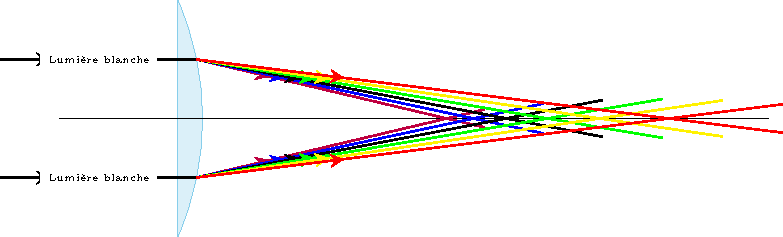
\includegraphics[width=.61\linewidth]{abbe_chroma.pdf}
		\captionsetup{justification=centering}
		\caption{Exemple (exagéré) de dispersion (aberration chromatique).}
		\label{fig:aberr}
	\end{figure}
}%

\end{document}
